\section{Simulation}
Using the SEPRAN package a simulation of the problem was made. First the mesh was defined, see Figure \ref{fig:empty_mesh}. The mesh is then uniformly filled with triangular elements, see Figure \ref{fig:filled_mesh}. The source code for this mesh is shown in appendix \ref{ap:mesh}.
\begin{Figure}
 \centerfloat
 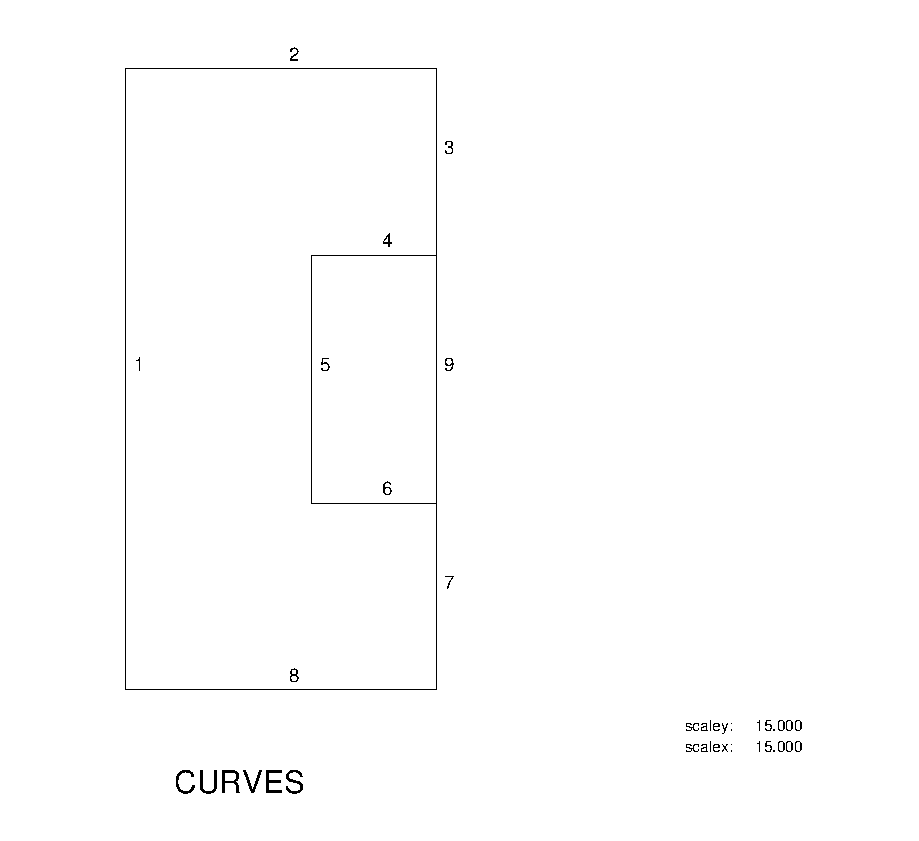
\includegraphics[width=0.4\linewidth, trim=1cm 2cm 7cm 0.5cm, clip]{empty_mesh.eps}
 \captionof{figure}{Mesh boundaries.}\label{fig:empty_mesh}
\end{Figure}

\begin{Figure}
 \centerfloat
 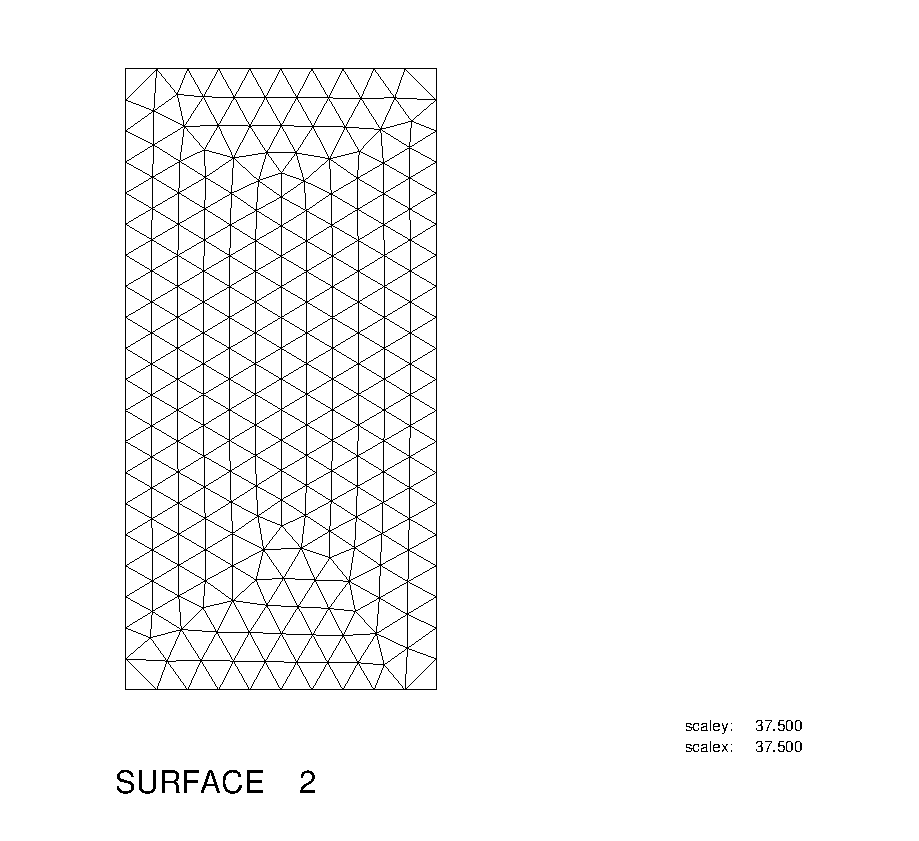
\includegraphics[width=0.4\linewidth, trim=1.5cm 2cm 7.5cm 0.5cm, clip]{filled_mesh.eps}
 \captionof{figure}{Mesh filled with triangular elements.}\label{fig:filled_mesh}
\end{Figure}

\begin{Figure}
 \centerfloat
 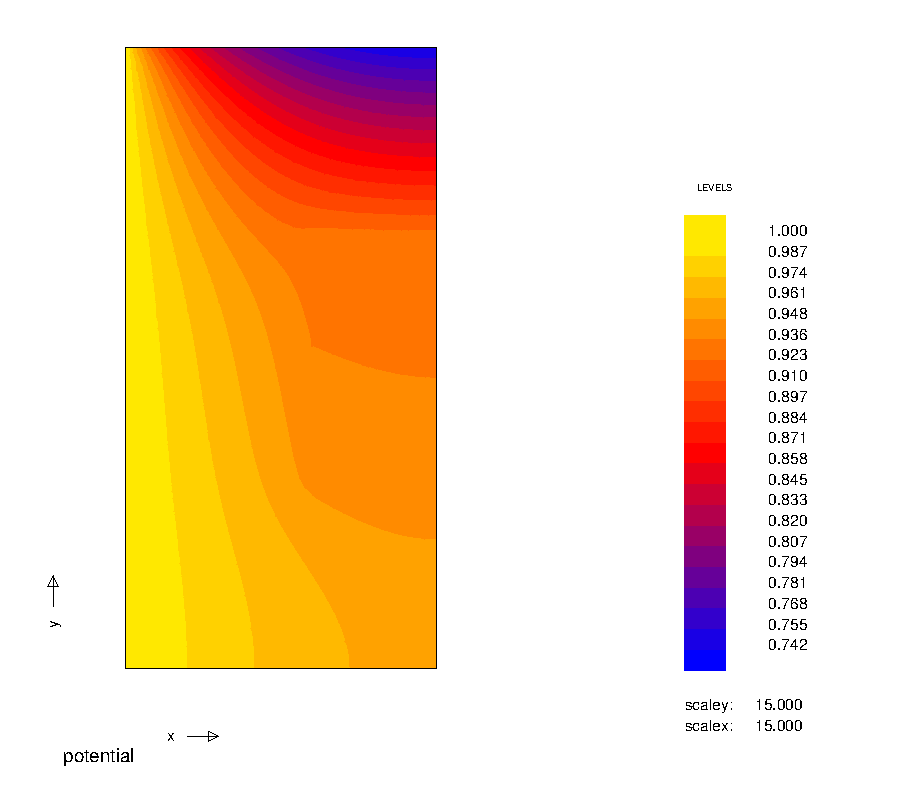
\includegraphics[width=0.8\linewidth]{coef_001.eps}
 \captionof{figure}{Heat distribution for $\alpha = 0.01$.}\label{fig:coef_0.01}
\end{Figure}

\begin{Figure}
 \centerfloat
 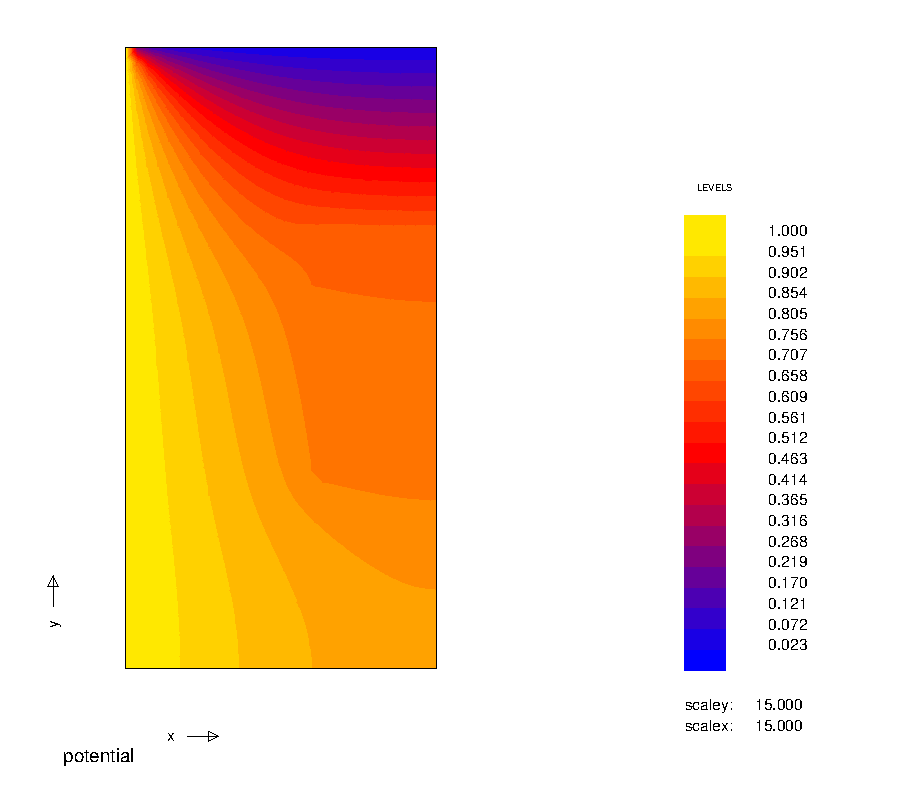
\includegraphics[width=0.8\linewidth]{coef_10.eps}
 \captionof{figure}{Heat distribution for $\alpha = 10$.}\label{fig:coef_10}
\end{Figure}